Um die sehr unterschiedlichen Implementierungen miteinander vergleichbar zu machen, werden Eigenschaften als Kriterien benötigt, die mehr oder minder auf jede einzelne zutreffen und relevant für den wirtschaftlichen Betrieb einer \gls{BC} sind.
%~ Diese Kriterien auch sollen relevant für den Anwendungsfall, eventuelle Einschränkungen und die Notwendigkeit zur .
Die Wertung soll klar von geringer Zielerfüllung zur höheren erkennbar sein.

%%
\section{Grundlegendes zur Informationstechnologie}\label{krit:it}

Grundsätzlich treffen diese Annahmen auch auf andere Wissensgebiete zu.
Allerdings ist die Bedeutung erst seit der Erfindung des Personal Computers und Zugang zum Internet für große Bevölkerungsteile durchsetzbar.
Gerade diese Parallele der Entwicklung des Internets zu dem Wandel den auch die \gls{BCT} bringen kann, ist der Grund hier auf eine Verbesserung des Zugangs und eine erneute Dezentralisierung abzuzielen.


\subsection{Offener Standard}\label{krit:openstandard}

Die Standardisierung einer Blockchain ist ein wesentlicher Bestandteil zur Sicherung der beabsichtigten Anwendungsfälle.
Sowohl die bisher getroffenen Entscheidungen als auch der Prozess für neue Entscheidungen sollten daher standardisiert sein um beurteilt oder in Zukunft an die Erfordernisse angepasst werden zu können.

Über einzelne \gls{BCI} hinweg bringt die Standardieirung auch Austauschmöglichkeiten wie \emph{Interledger} (\ref{first:interledger}), \gls{LN}\footnote{Whitepaper \autocite{p:lightning}} oder Comit~Network\footnote{Whitepaper \autocite{p:comit}}. Zur Zeit der Arbeit werden erste Live-Tests im Mainnet über drei Netzwerke verschiedener Implementierungen von hinweg durchgführt.
\subsection{Quelloffene Software}\label{krit:opensource}

%~ Zugänglichkeit
Einem Anwender kann nicht allgemeingültig zugetraut werden, die betrieblich zu nutzende Software selbst zu prüfen. Die betrieblichen Prozesse sollten aber ermöglichen Vertrauen in die IT-Umgebung zu induzieren. Das gilt insbesondere dann, wenn die verarbeiteten Daten ggf. ungewollt mit Dritten geteilt werden könnten.

Allein die Verfügbarkeit des Quellcodes ist daher für sich kein Mehrwert, den er nutzen kann.
Sofern allerdings Quellen zur Verfügung stehen, kann u.a. über einen reproduzierbaren Build-Prozess (engl. reproducable build) und digitale Signaturen der Binärdateien sichergestellt werden, dass die ausgeführte der Software auch aus dem verfügbaren Quellcode resultierte.

Sobald Anpassungen an einer Software notwendig werden, ist die Verfügbarkeit des Quellcodes aber ein entscheidendes Kriterium dazu unter Einsatz von begrenzten Ressourcen befähigt zu sein.\footnote{Selbst Herstellern kommt Quellcode abhanden \autocite{w:ms-binpatch}}
Auch bei Anpassungen durch den Hersteller kann damit nachvollzogen werden ob die angekündigten Änderungen gemacht wurden oder ggf. ein Problem unscharf formuliert oder gar verschwiegen wurde.

Dieser Vertrauensanker bewirkt, dass wir erkennen können wie und warum etwas funktioniert.
So wie Geometrie verstanden und angewendet werden kann, wenn ein gutes Buch die Grundlagen darlegt.

\subsection{Entwicklungsstand}\label{krit:entwicklungsstand}

Für die Anwendbarkeit einer Blockchain-Implementierung sind Stabilität und umgesetzte Features eine gute Maßgabe.


\subsection{Schnittstellen}\label{krit:schnittstellen}

Sofern eine Blockchain-Implementierung nicht genau auf den eigenen Anwendungsfall zugeschnitten ist, stellt sich die Frage welche Anpassungen notwendig werden.
Anpassungen sind auf Seiten des neuen Informationssystems oder auf der des alten denkbar.
Um die bisherigen Prozesse nicht zu gefährden, ist grundsätzlich die Anpassung des neuen Systems oder die Schaffung von Adaptern zwischen den Schnittstellen zu empfehlen.

\subsection{Anpassbarkeit}\label{krit:anpassbarkeit}

Die Verfügbarkeit von Schnittstellen ist für die Schaffung dieser Adapter ausschlaggebend.
Sofern keine nutzbaren Schnittstellen vorhanden sind, stellt sich die Frage wie leicht diese geschaffen werden können.
Auch bei fehlenden Funktionen ist es von wesentlichem Vorteil wenn 

\subsection{Community}\label{krit:community}

Die Unterstützung einer Software hängt wesentlich von der Unterstützung durch Nutzer ab.\footnote{\enquote{The Importance of Having Users} \autocite{Raymond:CB}} Bei prorietären Produkten leuchtet dies direkt ein, da die Lizenzeinnahmen die Finanzierung der Entwicklung ermöglichen. Wir haben aber beim Kriterium \nameref{krit:opensource} festgestellt, dass gerade in Systemen die auf Vertrauen basieren, die Umsetzung als Offener Standard und Freie Softwarelizenzen ein ausschlaggebendes Argument im Wettbewerb darstellen. 
Dabei geht es nicht nur um den Wettbewerb um die Nutzer, die eventuell Fehler melden und die Entwicklung durch Mitwirkung oder durch freiwillige monetäre Leistungen unterstützen. Es geht insbesondere auch um die Entwicklergemeinschaft, die Beiträge zur fraglichen Software leisten. Dazu zählen auch solche die keine Programmierung, sondern eventuell Übersetzungen, Dokumentation und Werkzeuge im Umfeld schaffen.

Der kritischste Teil der Community sind aber die Personen, die den Kern des Projektes stellen. Ein Team mit nur einem Entwickler ist mit einem höheren Ausfallrisiko zu bewerten als ein Team aus zehn Entwickler. Selbst wenn der einzelne Entwickler initial besser Leistungen erbringt bleibt sein Ausfall eine Bedrohung für den Fortbestand des Projektes für solche Nutzer die dringende Problemfälle nicht selbst meistern können.

\subsection{Dokumentation und Werkzeuge}\label{krit:werkzeuge}

In wie weit eine \gls{BCI} leicht nutzbar gemacht werden kann hängt stark davon ab wie leicht es Neulingen gemacht wird sich diese zu eigen zu machen.
Dazu sind Werkzeuge und Dokumentation wie Beispiele enorm hilfreich.

\section{Blockchain-bezogene Eigenschaften}\label{krit:blockchainproperties}

\subsection{Konsens}\label{krit:consensus}

Der Konsensmechanismus  \emph{Paxos}, der bei \nameref{impl:hyperledger} verwendung findet, wurde mittels Voting geschaffen. Bei Bitcoin und Ethereum ist es derzeit ein \gls{PoW}. Ethereum hat einen kontinuierlichen Change-Prozess und eine Roadmap auf der der Wechsel zu einem \gls{PoS}
vorgesehen ist und zumindest für konsortiale Instanzen einer \gls{BC} ist ein reines Signing z.B. mit Ethereum oder Quorum konfigurierbar. Im folgenden sollen die gefundenen Mechanismen vom schwächsten zum stärksten hinsichtlich der Sicherheitsleistung benannt werden.
Künftige Neuentwicklungen können hier entsprechend eingefügt werden.

Signing (engl. Unterzeichnen) ist die schwächste Form einen Konsens zu Erreichen. Der Ansatz bricht mit dem Ziel Autoritäten zu ersetzen.
Ein Teilnehmer in der Rolle eines \emph{Signers} bestimmt %abgesehen von der
allein über den Konsens eines Blockes.

Die Auswirkung von Voting ist die Notwendigkeit zur Akkreditierung der Stimmberechtigen, das Vertrauensproblem bleibt bestehen und wird nur vom Gegenstand des Votings auf das Voting selbst übertragen. Unter der Annahme, dass jeder Stimmberechtigte alles über die anderen weiß, ist auch ein virtuelles Voting denkbar.\footnote{\emph{Hashgraph} \autocite{p:hashgraph}} Damit wäre das Vertrauensproblem bei der Entscheidungsfindung keine Problem mehr, das Problem zur Akkreditierung wird aber nicht gelöst und um Bandbreite und Netzwerkverzögerung bereichert. Daher funktioniert der Ansatz bisher nur mit Einschränkungen\footnote{\url{https://www.reddit.com/r/hashgraph/comments/79g4po/hashgraph_is_not_a_blockchain_proofofwork/}  \autocite{w:reddit}} verbunden. Insb. müssen zwei drittel der Teilnehmer ehrlich bleiben.

Für \gls{PoS} wird eine bestimmte Mindestmenge an nativen Währungseinheiten als Sicherheitsleistung für hinterlegt. Der Teilnehmer, der den Block erstellen darf und den Ausgabeaufschlag erhält muss zufällig ermittelt werden. Falls ein Teilnehmer einen vom Konsens abweichenden Block produziert ist seine Sicherheitsleistung für ihn verloren. Es ist beabsichtigt dies bei Ethereum ab der Phase~4 \enquote{Serenity Release} einzuführen.\footnote{\enquote{Die Phasen von Ethereum} \url{https://etherbasics.com/basics/ethereum-phasen/}}. Ein Voting kann ebenfalls ein \gls{PoS} darsstellen, indem z.B. statt Währungseinheiten die Stimmberechtigung als Sicherheitsleistung verwendet wird. Der wesentliche Grund für das Verfahren ist der dann ausbleibende hohe Energieverbrauch bei \gls{PoW} und die Eignung für erlaubnisfreie, globale \gls{BC}.
%\footnote{ \autocite{p:pos:ouroboros}} \autocite{p:tendermint}

Beim Ansatz von Bitcoin, dem \gls{PoW}, wird durch laufendes Hashing alternativer Kombinationen der Transaktionen und Metadaten für einen nächsten Block ein Ziel gesucht, das der algorithmisch vorgegeben \gls{glos:Schwierigkeit} im Netzwerk entspricht oder größer als diese ist. Dabei wird eine globale Konkurrenz um den \gls{glos:Ausgabeaufschlag} aufgebaut. Als Folge der Konkurrenzsituation in Verbindung mit der Steigerung des Wertes nativer Währungen -- insb. bei Bitcoin, Ethereum und Monero -- ist in der Vergangenheit der Energiebedarf ständig angestiegen. Teilnehmer, die bei dem Wettlauf nicht mithalten können, haben keine Möglichkeit den Konsens\footnote{Denkbar ist Zensur von Transaktionen durch aktives Verschweigen.} zu beeinflussen.

\subsection{Erlaubnisfreiheit}\label{krit:erlaubnisfreiheit}

Diese Eigenschaft besagt, ob der Zugang als Teilnehmer ohne Akkreditierung möglich ist.
Der Fall unterschiedlicher Rollen unter den Teilnehmern muss hier vergleichend betrachtet werden.

%~ \subsection{Vertrauenslosigkeit}\label{krit:vertrauenslosigkeit}

%~ Die frage nach Autoritäten ist immer eine Frage nach Vertrauen. Im Unternehmensumfeld lässt dies auch das Eigentum am Geschäft bezweifeln.
%~ In diesem Fall ist zwischen den verschiendenen \gls{BCI} keine entscheidende Abstufung erkennbar.
%~ Daher wird diese Bewertung einstweilen als binär angenommen.

\subsection{Programmierbarkeit}\label{krit:programmierbarkeit}

Die Möglichkeit des programmierbaren Geldes kann nicht nur binär betrachtet werden.
Aber sie ist notwendig dem Protokoll inhärent. Die Programmierung in einer weiteren Schicht (engl. 2nd Layer) außerhalb des Konsensprotokolles ist davon unberührt.
Ausgenommen werden an dieser Stelle Eigenschaften wie Sprachkonzepte oder konkrete Unterstützung bezüglich der \gls{IDE} -- s.a. \nameref{krit:werkzeuge}.
Dagegen betrachtet werden muss die Turingvollständigkeit, also ob jedes berechenbare Problem zumindest theoretisch gelöst werden kann.  
%~ sofern der jeweiligen \gls{BCI} inhärent

%~ \subsection{Kapazität}\label{krit:kapazitaet}

%~ Die Blockgröße

\subsection{Interchain-Unterstützung}\label{krit:interchain}

\subsection{Native Währung}\label{krit:waehrung}

Eine \gls{BC} kann für ihr Anreizsystem eine native Währung einsetzen.
Für den Unternehmenseinsatz kann dies je nach Jurisdiktion ein zusätzlicher Aufwand sein.
Vorgaben hierzu können geändert werden,  Anpassungen an eine Regulierung und im schlimmsten Fall die Außerbetriebnahme der \gls{BC} notwendig machen.

\subsection{Fungibilität}\label{krit:fungibility}

Diese Eigenschaft beschreib die gleichwertigkeit bzw. Austauschbarkeit der nativen Währungseinheiten.
Die native Währung betreffend ist interessant, ob die Einheiten eines Teilnehmers von denen eines anderen Teilnehmers unterschieden werden können.
Transparenz der Besitzverhältnisse eines Teilnehmers bedeutet auch, dass diesem -- und anderen über Transaktionen mit ihm in Verbindung stehenden Teilnehemrn -- weitere Eigenschaften zugeordnet werden können. Damit können ggf. agierende Personen identifiziert werden oder eine \enquote{Verschmutzung} von Währungseinheiten begründet werden.

\subsection{Transaktionsgeschwindigkeit}\label{krit:transaktionsgeschwindigkeit}

Die Frage nach Performance ist eine naheliegende Entscheidungsgrundlage bei der Beschaffung von IT-Systemen.
Benchmarks zum Vergleich verschiedener \gls{BCI} stellen gerne auf die \gls{TPS} ab.
Die Vergleichbarkeit ist aber nur bedingt gegeben, da Blockgröße und Transaktionsgröße abhängig von den Vorgaben sehr starke Unterschiede aufweisen können.
Zusätzlich unterscheidet sich die Transaktionsgröße für verschiedene Anwendunsgfälle sehr stark.
Eine pauschale oder durchschnittliche Angabe sollte daher nicht die primäre Grundlage für eine Entscheidung sein.

%~ \subsection{Periode und Stetigkeit der Blockzeit}\label{blocktime}

%~ An dieser Stelle wird zur Veranschaulichung auf die beiden großen öffentlichen, globalen Blockchains Bitcoin und Ethereum ausgewichen.
%~ % Ähnliche Auswirkungen sind mit privaten \gls{BC} nicht unbedingt zu beobachten.

%~ Die Blöcke werden im Fall von \gls{PoW} Blockchain, wie Bitcoin und Ethereum, in statistisch gleichen großen Periode erschaffen. Am Bsp. Bitcoin wird diese statistische Periode von 10~Minuten am Graphen sehr deutlich erkennbar fast ständig unterschritten. Dieser Umstand hat abhängig von der \gls{glos:Hashrate} auch ein schnelleres Voranschreiten des \gls{glos:Halfing}s zur Folge, als es ursprünglich prognostiziert wurde.

%~ U.a. über die Website \href{https://bitinfocharts.com/comparison/bitcoin-confirmationtime.html}{bitinfocharts.com} können insb. zum Projektstart starke Schwankungen beobachtet werden. Dies lässt sich über die geringe Anzahl der Teilnehmer zu diesem Zeitpunkt erklären.
%~ Weitere Schwankungen kennzeichnen problematische Ereignisse in der globalen Blockchain wie Schwierigkeiten von dominierenden Marktteilnehmern (Bsp. \gls{glos:Exchange}), staatliche Regulierung und medialer Hype oder einfach nur Schwankungen im Preis\footnote{Bsp. 12.\,November~2017 Kurzzeitiger Einbruch um ca.\,20\,\% \autocite{w:bitcoinde-kurs}} die mit solchen Ereignissen und der Schwierigkeit im Netzwerk korrelieren.
%~ % Ähnliches ist also auch im Unternehmenseinsatz bei Updates zu erwarten, die nicht gleichzeitig 

%~ \begin{figure}
%~ 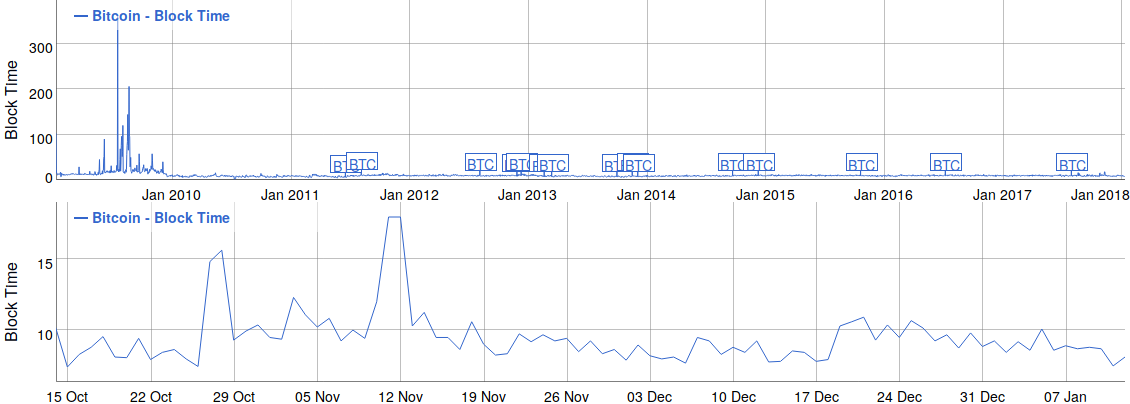
\includegraphics[width=\textwidth]{img/bitinfocharts-blocktime-btc}
%~ \caption[blocktime-btc]{\label{blocktime-btc}\mbox{Blockzeit f. Bitcoin}, \mbox{oben: Gesamt}, \mbox{unten: 6~Monate} %
%~ \mbox{Quelle: \cite{w:bitinfocharts}}
%~ } %\footnote{\url{https://bitinfocharts.com/comparison/bitcoin-confirmationtime.html}}
%~ \end{figure}

%~ Am Bsp. Bitcoin Abb.\,\ref{blocktime-btc} ist neben der Anfangsphase mit wenigen Teilnehmern eine stetige Schwankung über die Gesamte Laufzeit erkennenbar.

%~ Hierzur ist  zu sagen, dass eine größere Schwankung die geringere Wertung nach sich zieht,
%~ allerdingdings können die 

%~ \begin{figure}
%~ 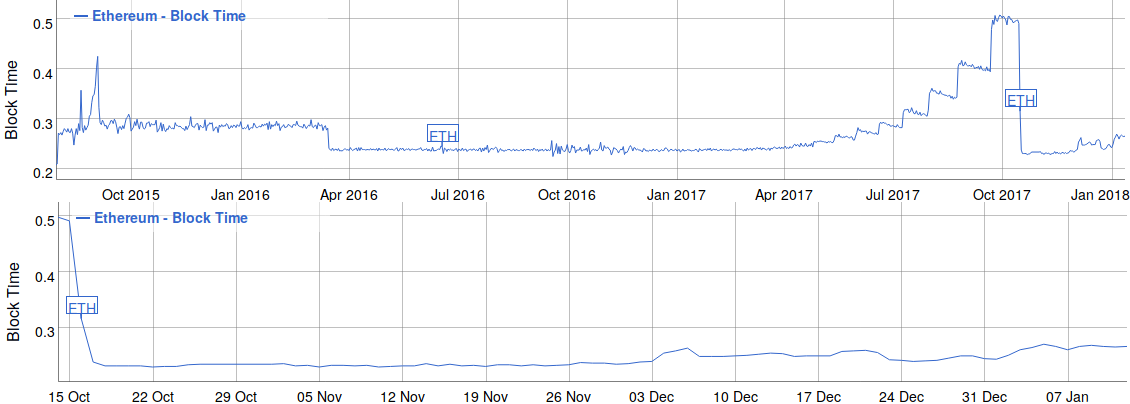
\includegraphics[width=\textwidth]{img/bitinfocharts-blocktime-eth}
%~ \caption[blocktime-eth]{\label{blocktime-eth}\mbox{Blockzeit f. Ethereum}, \mbox{oben: Gesamt}, \mbox{unten: 6~Monate} %
%~ \mbox{Quelle: \cite{w:bitinfocharts}}
%~ } %\footnote{\url{https://bitinfocharts.com/comparison/bitcoin-confirmationtime.html}}
%~ \end{figure}

%~ Bei Ethereum Abb.\,\ref{blocktime-eth} tritt eine ähnliche Auffälligkeit zur Anfangsphase auf.
%~ Zusätzlich sind sehr Deutlich Auswirkungen im März~2016\footnote{Homestead Release am 14.\,März~2016 \autocite{w:etherchain-hardforks}} und das Einsetzen der \enquote{Schwierigkeits-Bombe} (Engl. Difficulty-Bomb) bis zum abrupten Abfall\foornote{ab April~2017 (am Graph abgelesen) bis zum Byzantium Release am 16.\, Oktober~2017 \autocite{w:etherchain-hardforks}}. Beide Änderungen stehen je mit einer \gls{glos:Hard~Fork} in Verbindung.

%\begin{figure}
%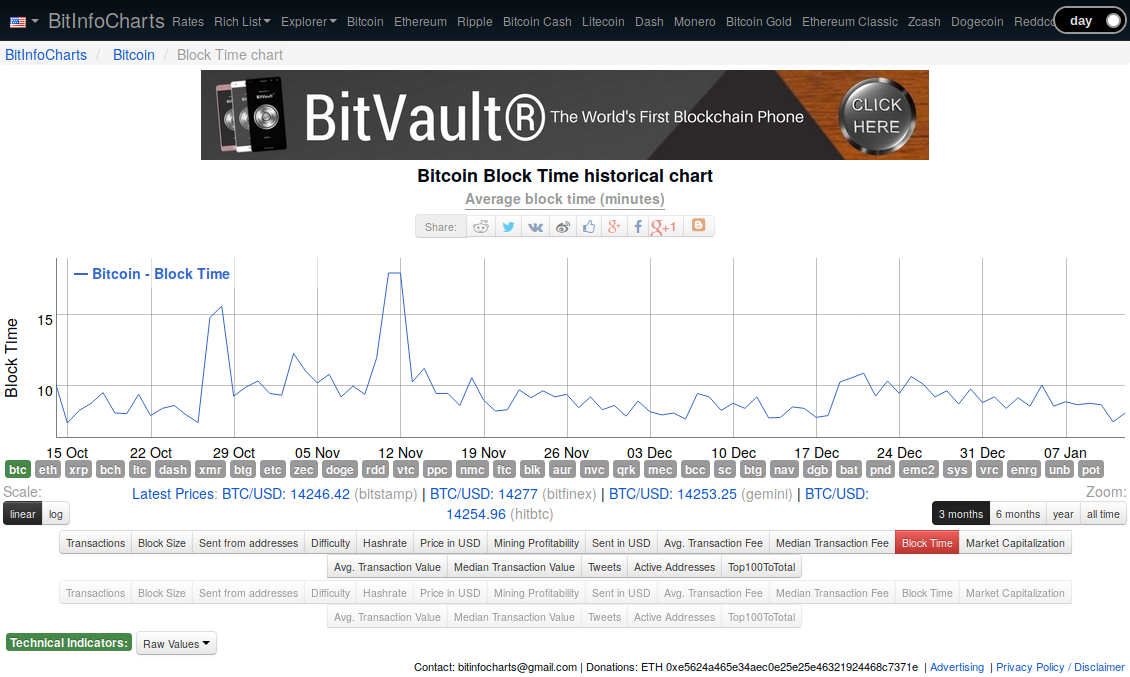
\includegraphics[width=\textwidth]{img/screenshot-bitinfocharts-2018-01-13-18-27-38}
%\end{figure}

%~ https://etherscan.io/chart/blocktime

%~ + Entwicklung von Kriterien
  %~ + Welche Eigenschaften bieten die Implementierungen
	%~ * Unterstützung
	%~ * Entwicklungsstand
	%~ * Kosten
	%~ * 
  %~ + Welchen Anwendungsfällen sind sie zu-/abträglich
	%~ * Viele Transaktionen
	%~ * Privatsphäre
	%~ * Integration Bestehender IT

%%
\section{Wirtschaftliche Gesichtspunkte}\label{krit:oeconomics}

Bevor naheliegende Kosten betrachtet werden, soll auch auf die Ertragsseite der Wirtschaftlichkeoitsbetrachtung hingewiesen werden.
Die Bewertung ist sehr stark vom Einzelfall mit vielen Einflussfaktoren 
abhängig und wird daher nicht als Kriterium aufgenommen.
Was Wertung von Angaben zu Kosten und Erträgen angeht, so sind höhere Kosten immer schlechter zu werden und höhere Erträge besser.

\subsection{Personalverfügbarkeit}\label{krit:personal}

Noch heute erscheint die Neuerung durch die \gls{BCT} so groß, dass der Bedarf an Personal nicht gedeckt ist.
%Aber ähnlich die Geometrie sind die Kenntnisse dahinter nur auf Zeit Spezialwissen.
Umso mehr Anwendungen den Alltag beeinflussen, umso mehr Informationen öffentlich zugänglich sind, desto leichter wird es sein diese Kompetenzen am Markt zu erhalten.
Bisweilen haben Firmen aber genau das Problem ihren Bedarf am Markt zu decken.

Die Betrachtung stellt auf die Verfügbarkeit von Personal und damit die Durchführbarkeit beabsichtigter Projekte ab und beinhaltet noch nicht die Kosten. 
%~ Daher spielt der Faktor Personal noch eine enorme Rolle bei initialen (horizontale Weiterbildung) und vor allem laufenden Kosten für Gehälter.
Die Wertung für geringere Personalverfügbarkeit ist kleiner als die höherer.

\subsection{Beschaffungskosten}\label{kosten}

%~ (gewonnen aus \nameref{first:kosten})
Für die Verwendung im konkreten Unternehmen notwendigen Einmalaufwendungen können eine wesentliche Zugangshürde zu Technologie darstellen.
Dies kann auch trotz \emph{Offener Standards} und Open~Source Software der Fall sein wenn einzelne Akteure ihre Position oder ihren Wissensvorsprung monetarisieren.
Initiale Kosten können insb. Anschaffung von Hardware und ggf. Lizenzkosten\footnote{Bsp. Softwarelizenzen, Lizensierung von Patenten; auch Konzessionen wie die \emph{BitLicense} \autocite{w:bitlicense}} darsellen.
Auch andere Einmalaufwendungen -- z.B. für den Zugang zu Verbänden -- zählen hierzu.

\subsection{Laufende Kosten}

Abgesetzt von den Beschaffungskosten sind auch laufende Kosten zu betrachten.
Hier insb. Beiträge zu Verbänden und auf die \gls{BCI} beziehbare Personalkosten (s.a. \ref{krit:personal}) wie Gehälter und Weiterbildung.

%~ (gewonnen aus \nameref{first:regulierung})
Abgesehen von den Kosten ist auch die Beeinflussung des Umfeldes durch
Standardisierung und Regulierung (\label{regulierung}s. \ref{first:regulierung}) für Unternehmen eine Herausforderung.
Dabei können Kosten unregelmäßig auftreten und unvorhersehbar auftreten.
